\documentclass[../main/main.tex]{subfiles}
\graphicspath{{./figures/}}

\makeatletter
\renewcommand{\@chapapp}{Travaux pratiques -- TP}
\makeatother

% \toggletrue{student}
% \toggletrue{corrige}
% \renewcommand{\mycol}{black}
\renewcommand{\mycol}{gray}

\begin{document}
\setcounter{chapter}{20}

\settype{enon}
\settype{solu_prof}
\settype{solu_stud}

\chapter{\cswitch{%
	  Correction du TP
  }{%
	  Dosages par titrages du vinaigre
  }
 }

\enonce{%
	\begin{prgm}
		\begin{tcb}*(ror)"know"{Savoir}
			\begin{itemize}
				\item Titrage direct
				\item Equivalence
				\item Indicateur coloré de fin de titrage
			\end{itemize}
		\end{tcb}
		\begin{tcb}*(ror)"how"{Savoir-faire}
			\begin{itemize}
				\item Mettre en œuvre une réaction acide-base pour réaliser une
				      analyse quantitative en solution aqueuse.
				\item Identifier et exploiter la réaction support du titrage
				      (recenser les espèces présentes dans le milieu au cours du
				      titrage, repérer l'équivalence, justifier qualitativement
				      l'allure de la courbe ou le changement de couleur observé).
				\item Exploiter une courbe de titrage pour déterminer la
				      concentration d'une espèce dosée.
				\item Choisir et utiliser un indicateur coloré de fin de
				      titrage~; distinguer l'équivalence et le virage d'un indicateur
				      coloré de fin de titrage.
				\item Titrage par suivi conductimétrique et pH-métrique
			\end{itemize}
		\end{tcb}
	\end{prgm}
	\vspace{-10pt}

	\section{Objectifs}

	\begin{itemize}
		\item Revoir le protocole de dilution.
		\item Revoir le protocole expérimental de pH-métrie~; Tracer des courbes
		      pH-métriques grâce à Régressi ou Latispro.
		\item Choisir un indicateur coloré acido-basique.
		\item Comprendre le principe de la conductimétrie et connaître les formules.
		\item Revoir le protocole expérimental de conductimétrie~; Tracer des
		      courbes conductimétriques grâce à Régressi ou Latispro.
		\item Exploiter une équivalence pour déterminer le degré alcoolique d'un
		      vinaigre.
		\item Évaluer une incertitude lors de mesures avec des appareils de
		      tolérance connue.
		\item Évaluer une incertitude de mesure dans laquelle interviennent
		      plusieurs sources d'erreurs.
	\end{itemize}

	\section{S'approprier}
	\subsection{Introduction}

	On cherche à déterminer le degré d'un vinaigre par titrage pH-métrique et
	conductimétrique, à partir d'une solution d'hydroxyde de sodium (soude)
	(\ce{Na+}~; \ce{OH-}). Un vinaigre est essentiellement une solution aqueuse
	diluée d'acide éthanoïque (ou acétique) de formule \ce{CH3COOH}. Les
	concentrations commerciales sont exprimées en degrés. Le degré d'un vinaigre
	correspond à la masse (en gramme) d'acide éthanoïque pur contenu dans
	$\SI{100}{g}$ de vinaigre.

	\begin{tcb}(data){Données utiles}
		\begin{itemize}
			\item Masses molaires~: $M(\ce{H}) = \SI{1,0}{g.mol^{-1}}$, $M(\ce{O}) =
				      \SI{16,0}{g.mol^{-1}}$ et $M(\ce{C}) = \SI{12,0}{g.mol^{-1}}$
			\item Masse volumique du vinaigre~: $\rho_V \approx \SI{1,0}{g.cm^{-3}}$
			\item Couples acido-basiques mis en jeu~: \ce{H2O/OH-} (pK$_A = 14$) et
			      \ce{CH3COOH/CH3COO-} de pK$_A = \num{4,8}$.
		\end{itemize}
	\end{tcb}

	\subsection{Principe d'un pH-mètre}

	Un pH-mètre est constitué de deux électrodes~: une électrode de verre de
	potentiel d'électrode proportionnel au pH de la solution dans laquelle elle
	trempe et une électrode de référence (pour laquelle le potentiel d'électrode est
	fixe). Ces deux électrodes constituent une pile électrochimique et un
	millivoltmètre mesure la force électromotrice $e$ de cette pile, qui est une
	fonction affine du pH~: $e = a + b \rm pH$ où $a$ et $b$ sont deux constantes
	qui dépendent de la nature des électrodes et de la température. Avant toute
	mesure, il faut donc étalonner le pH-mètre.

	\subsection{Le principe de la conductimétrie}

	Cette méthode repose sur l'existence d'ions en solution et sur leur capacité à
	faciliter le passage d'un courant. La nature des ions et leurs concentrations
	modifient la conductance $G$ du système (grandeur qui est l'inverse de la
	résistance $R$) exprimée en \si{S} (Siemens). Plus le milieu est propice au
	passage du courant, plus la conductance est élevée. Celle-ci est reliée à trois
	paramètres principaux~:

	\begin{tasks}[label=\arabic*)](3)
		\task la conductivité $\sigma$ du système
		\task la longueur $\ell$
		\task la section $S$ de la cellule
	\end{tasks}
	\begin{gather*}
		\beforetext{La conductance s'exprime alors selon}
		G = \frac{\sigma S}{\ell}
	\end{gather*}

	Ainsi, on ne parle pas de conductance \cancel{de la solution}, puisque la
	conductance dépend de la cellule de mesure et de sa géométrie. L'unité de
	conductivité est le $\si{S.m^{-1}}$~; le quotient $K = \ell / S$ est appelé
	constante de cellule. Ainsi, on a $G = \sigma / K$. La mesure de la conductance
	s'effectue avec un conductimètre, qui est en fait un ohmmètre.\bigbreak

	La conductivité $\sigma$ de la solution peut alors s'exprimer par la \textbf{loi
		de Kohlrausch}, exprimée sous une forme avec la chage de l'ion~:
	\begin{tcb}(prop){Loi de \textsc{Kohlrausch}}
		\[\boxed{\sigma = \sum_{i} \lambda_i \left|z_i\right| [{\rm X}_i]}\]
		\begin{itemize}
			\item $\lambda_i$ la conductivité molaire ionique de l'ion ${\rm X}_i$ (en
			      $\si{S.m^2.mol^{-1}}$) donnée dans les tables
			\item $z_i$ la charge de l'ion ${\rm X}_i$
			\item $[{\rm X}_i]$ la concentration de l'ion ${\rm X}_i$ en
			      $\si{mol.m^{-3}}$ (\textbf{Attention~!!})
		\end{itemize}
	\end{tcb}

	\begin{tcb}(impo)<lftt>'l'{Important}
		\begin{center}
			\bfseries
			La conductivité $\sigma$ de la solution prend en compte tous les ions
			présents dans la solution. Il faut donc faire l'inventaire des ions en
			solution avec soin, y compris les ions spectateurs.
		\end{center}
		La conductivité $\sigma$ évoluera donc lorsque la concentration des ions
		changera \textbf{ou} lorsque leur nature (et donc leur conductivité molaire
		ionique) changera. Et si le volume total de la solution peut être considéré
		constant, $\sigma$ sera une \textbf{fonction affine du volume versé lors
			d'un dosage}, la pente étant fonction des conductivités molaire ionique de
		chacun des ions qui apparaissent/disparaissent. \textbf{C'est pourquoi, on
			réalisera ce dosage avec un excès d'eau distillée}, pour pouvoir supposer le
		volume invariant par apport de solution titrante.
	\end{tcb}
}

\section{Analyser}
\subsection{Étude générale du dosage}

\setlist[blocQR,1]{leftmargin=10pt, label=\clenumi}
\QR{%
	Écrire l'équation du dosage, calculer la constante de la réaction
	en fonction des pK$_A$ et conclure sur la pertinence (est-elle
	totale~?) de cette réaction comme réaction de dosage.
}{%
	\leavevmode\vspace*{-30pt}\relax
	\begin{gather*}
		\ce{CH_3COOH\aqu{} + HO^-\aqu{} -> CH_3COO^-\aqu{} + H_2O\liq{}}
		\tag*{$K$}
		\\
		\Ra
		K =
		\frac{[\ce{CH_3COO-}]\ind{eq}c^\circ}
		{[\ce{HO-}]\ind{eq}[\ce{CH_3COOH}]\ind{eq}}
		\times \frac{[\ce{H_3O+}]\ind{eq}}{[\ce{H_3O+}]\ind{eq}}
		\Lra
		\boxed{K = \frac{K_A}{K_e}}
		\Ra
		\xul{K = 10^{\num{9.25}} \gg 1}
		\quad \text{donc totale}
	\end{gather*}
}

\QR{%
	Pourquoi peut-on suivre ce dosage par pH-métrie~? par
	conductimétrie~?
}{%
	Il y aura une variation brusque du pH, étant donné qu'avant l'équivalence on
	on a de l'acide à un $\pH \approx \pk$, et après on a des ions hydroxde donc
	le $\pH \approx \numrange{11}{12}$.
}

\QR{%
	\begin{minipage}[t]{0.80\linewidth}
		Sur l'étiquette de la bouteille de soude caustique, on peut voir
		ce pictogramme~: que signifie-t-il~? Quelles précautions faut-il
		prendre~?\\
		Vous pourrez consulter~\url{http://www.inrs.fr/media.html?refINRS=ED\%204406}
	\end{minipage}
	\hfill
	\begin{minipage}[t]{0.15\linewidth}
		\vspace{-10pt}
		$\underset{\text{Soude}}{\ghspic{acid}}$
	\end{minipage}
}{%
	Ronge~: gants et lunettes.
}

\subsection{Préparation de la solution $S_1$ à doser}

\enonce{%
	On souhaite doser $V_A = \SI{10}{mL}$ de vinaigre à partir d'une solution
	d'hydroxyde de sodium ou soude de formulation une fois dissociée dans l'eau
	(\ce{Na+}~; \ce{HO-}) et de concentration $c_B = \SI{1,0e-1}{mol.L^{-1}}$. On
	utilisera la burette sortie sur la paillasse ($\SI{25}{mL}$).
}

\QR{%
	Le vinaigre que nous utilisons a un degré alcoolique de 8. Peut-on
	utiliser directement la solution commerciale ou faut-il la diluer~? Si
	oui dans quelles proportions~? Expliquer, dans ce cas, votre protocole
	expérimental.
}{%
	\sswitch{
		\leavevmode\vspace*{-45pt}\relax
	}{
		\leavevmode\vspace*{-20pt}\relax
	}
	\begin{gather*}
		n_{\ce{CH3COOH},0} = \frac{m_{\ce{CH_3COOH},0}}{M(\ce{CH_3COOH})}
		\Ra
		c_0 = \frac{m_0}{MV\ind{V}}
		% \\\Lra
		\Lra
		\boxed{c_0 = \frac{m_0 \rho_V}{M m\ind{V}}}
		% \mathrlap{
		\qav
		\left\{
		\begin{array}{rcl}
			m_0      & = & \SI{8}{g}
			\\
			\rho_V   & = & \SI{1.0e3}{g.L^{-1}}
			\\
			M        & = & \SI{60}{g.mol^{-1}}
			\\
			m\ind{V} & = & \SI{100}{g}
		\end{array}
		\right.
		% }
		\\
		\AN
		\xul{
			c_0 = \SI{1.3}{mol.L^{-1}}
		}
		\\
		\beforetext{Équivalence~:}
		c_0V_A = c_B V\ind{equi}
		\Lra
		V\ind{equi} = \frac{c_0V_A}{c_B} = \xul{\SI{130}{mL}} \gg
		\frac{V\ind{bur}}{2}
	\end{gather*}
	Il faut donc \textbf{diluer par 10} pour avoir un volume équivalent aux
	alentours de \SI{13}{mL}.
	\begin{itemize}
		\item Prélever un peu ($\approx \SI{20}{mL}$) de vinaigre dans un bécher.
		\item Insérer \SI{10.0}{mL} de vinaigre dans une fiole jaugée de
		      \SI{100.0}{mL} à l'aide d'une pipette jaugée.
		\item Ajouter de l'eau jusqu'aux 3/4 puis mélanger.
		\item Compléter jusqu'au trait de jauge en prenant en compte le ménisque.
	\end{itemize}
}

\section{Réaliser}

\enonce{%
	\begin{tcb}[cnt, bld](impo){Important}
		Le port de la blouse fermée et des lunettes est obligatoire durant
		l'ensemble du TP. Les cheveux longs doivent être attachés, les lentilles
		de contact retirées, les jambes doivent être couvertes.
	\end{tcb}

	\subsection{Préparation de la solution $S_1$ à doser}

	\begin{itemize}[label=$\triangleright$]
		\item Préparer la solution $S_1$ selon le protocole que vous avez établi
		      dans la partie Analyser.
	\end{itemize}

	\subsection{Réalisation du dosage par pH-métrie}

	\begin{tcb}[bld, cnt](impo){Important}
		Attention, une sonde pH-métrique est très fragile (et très couteuse).
		Merci de manipuler avec beaucoup de précaution.
	\end{tcb}

	\subsubsection{Étalonnage du pH-mètre}

	\begin{tcb}[breakable](expe)<itc>{Étalonnage du pH-mètre}
		\begin{enumerate}
			\item La relation étant supposée linéaire (\textit{cf} S'approprier), il
			      suffit d'utiliser deux solutions étalon (solutions tampons à pH fixé)
			      afin d'avoir deux points de contrôle (une droite est définie avec
			      unicité par la connaissance de deux points). Le protocole est affiché
			      dans la salle en fonction des pH-mètres présents.
			\item Enlever les caches des électrodes et les rincer à l'eau distillée.
			\item Appuyer sur \texttt{cal}.
			\item Tremper les électrodes dans la solution pH = 7, puis à l'aide des
			      flèches, amener la valeur du pH sur 7, avant de valider. Certains
			      modèles s'autocalibrent, dans ce cas il suffit d'attendre.
			\item Rincer les électrodes entre les deux solutions tampon.
			\item Recommencer avec la 2\ieme\ solution tampon à pH = 4.
			\item Rincer de nouveau à l'eau distillée, puis appuyer sur mesure.
			\item Le pH-mètre est prêt à être utilisé~!
		\end{enumerate}
	\end{tcb}
}
\setcounter{subsection}{2}
\setcounter{subsubsection}{1}

\subsubsection{Dosage}

\enonce{%
	\begin{tcb}*(expe)<itc>"chem"{Dosage}
		\begin{enumerate}
			\item Remplir la burette avec la solution de soude. Purger la partie basse
			      de la burette (éliminer les éventuelles bulles d'air) et ajuster le
			      zéro de la burette. Il est impératif que la partie basse de la
			      burette contienne de la solution titrante, sinon vos mesures vont
			      être erronées.
			\item Rincer la pipette avec la solution $S_1$ de vinaigre préparée, puis
			      prélever $\SI{10}{mL}$ de cette solution et la mettre dans le bécher.
			      Ajouter environ $\SI{30}{mL}$ d'eau distillée de façon à ce que les
			      électrodes puissent tremper.
			\item Placer les électrodes de mesures dans le bécher et mettre l'agitation
			      magnétique en marche. \textbf{Attention, le barreau magnétique ne doit
				      pas toucher les électrodes}.
		\end{enumerate}
	\end{tcb}
}

\resetQ
\setlist[blocQR,1]{leftmargin=10pt, label=\sqenumi}
\QR{%
	Faire le schéma du montage sur votre compte-rendu.
}{%
	\hfill
	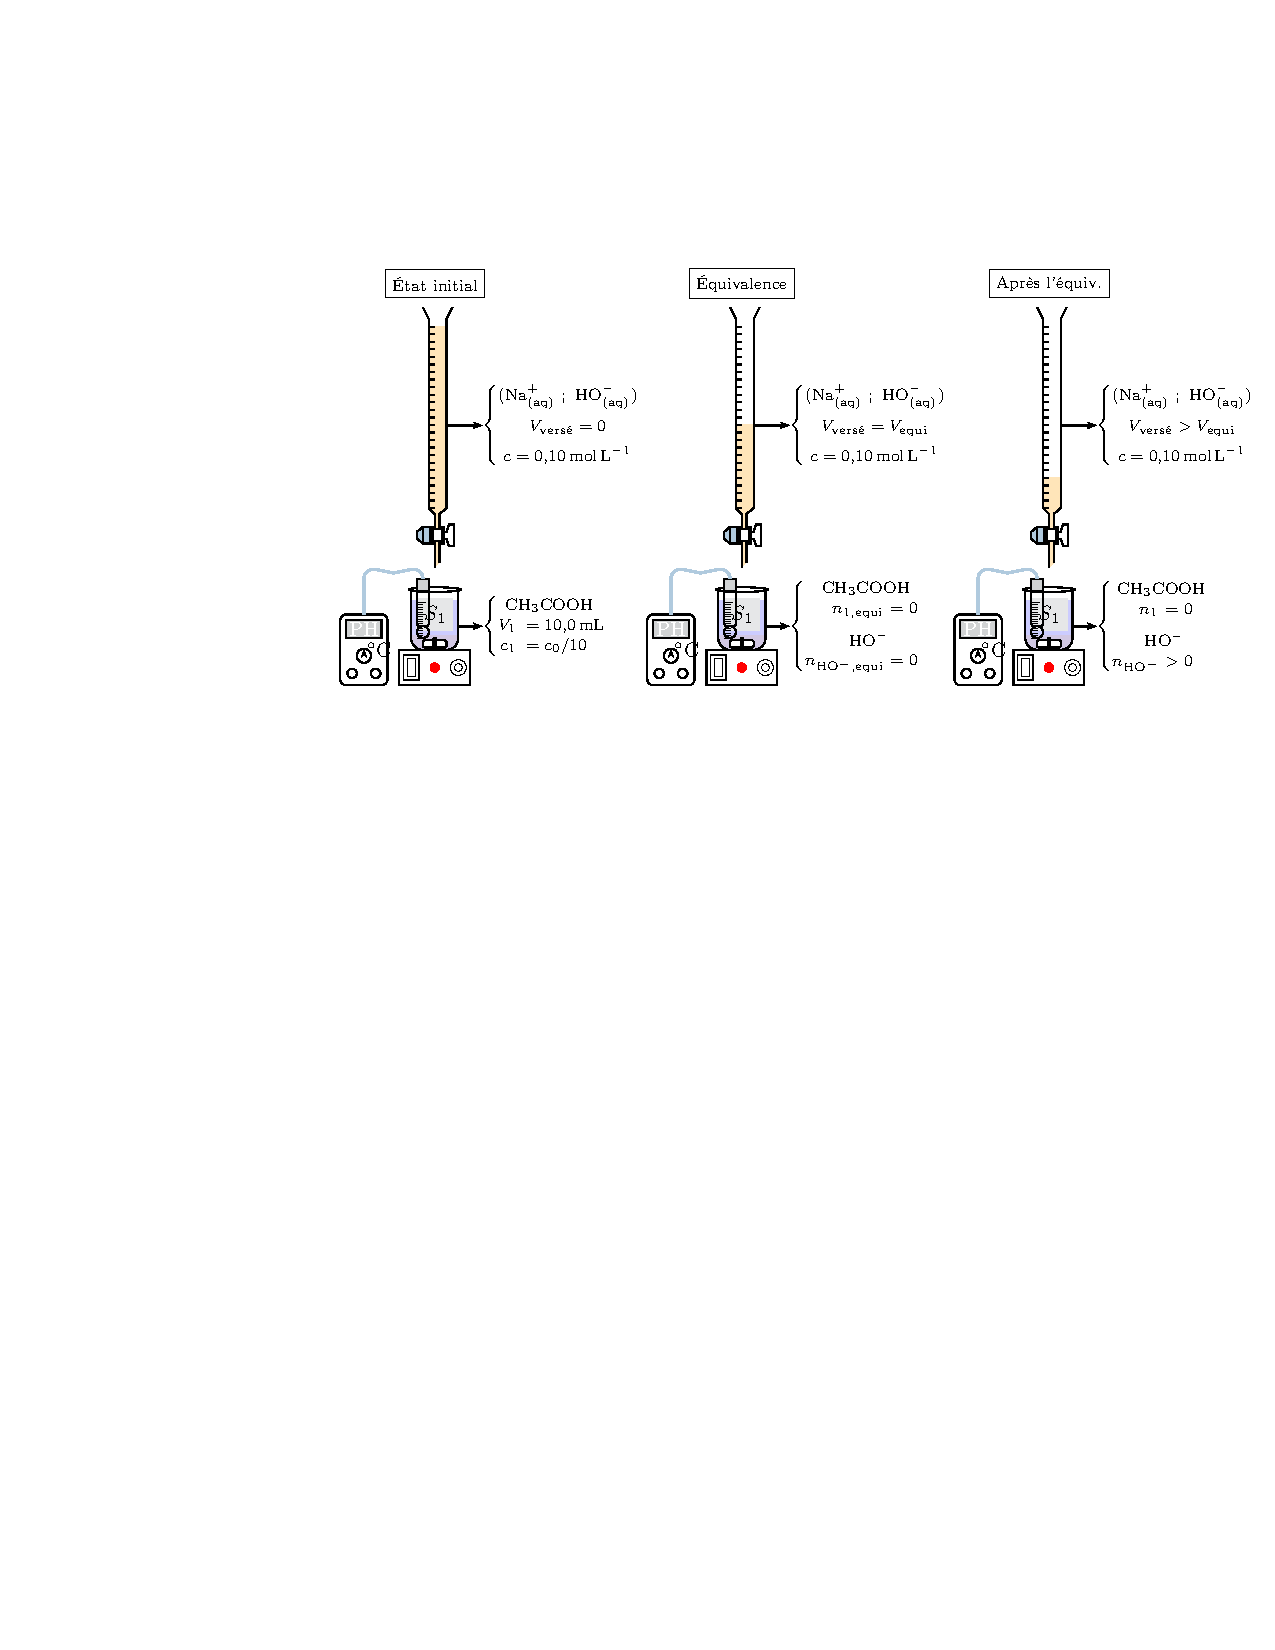
\includegraphics[width=.8\linewidth, valign=t]{vinaigre_verrie-fig1}
	\hspace*{\fill}
}

\QR{%
	Réaliser les mesures en remplissant un tableau de valeurs permettant
	de tracer $\pH = f(V_B)$, pour des additions de soude de $0,1,2… \si{mL}$
	jusqu'à ce que $V_B \approx 2 V_{B, \eqi}$.
}{%
	Non corrigé.
}

\subsubsection{Exploitation des mesures}

\enonce{%
	\begin{tcb}[breakable](expe)<itc>{Tracé de la courbe}
		\begin{enumerate}
			\item Allumer l'ordinateur sur votre session, puis ouvrir Régressi.
			\item Aller dans Fichier, nouveau, clavier et recopier votre tableau de
			      valeurs $(V_B~; \pH)$.
			\item Afficher le graphe $\pH = f(V_B)$. Relier les points expérimentaux
			      grâce aux options de graphe et réaliser un lissage d'ordre 3.
			\item Afin de déterminer l'équivalence, Regressi comporte directement la
			      méthode des tangentes. Dans le menu graphique, allez dans Outils
			      $\rightarrow$ tangente $\rightarrow$ méthode des tangentes (avec clic)
			      $\rightarrow$ cliquez sur un point juste avant ou juste après
			      l'équivalence.
		\end{enumerate}
	\end{tcb}
}

\QR{%
	Imprimer la courbe et relever le volume de soude versé à
	l'équivalence~: $V_{B, \eqi}$.
}{%
	\hfill
	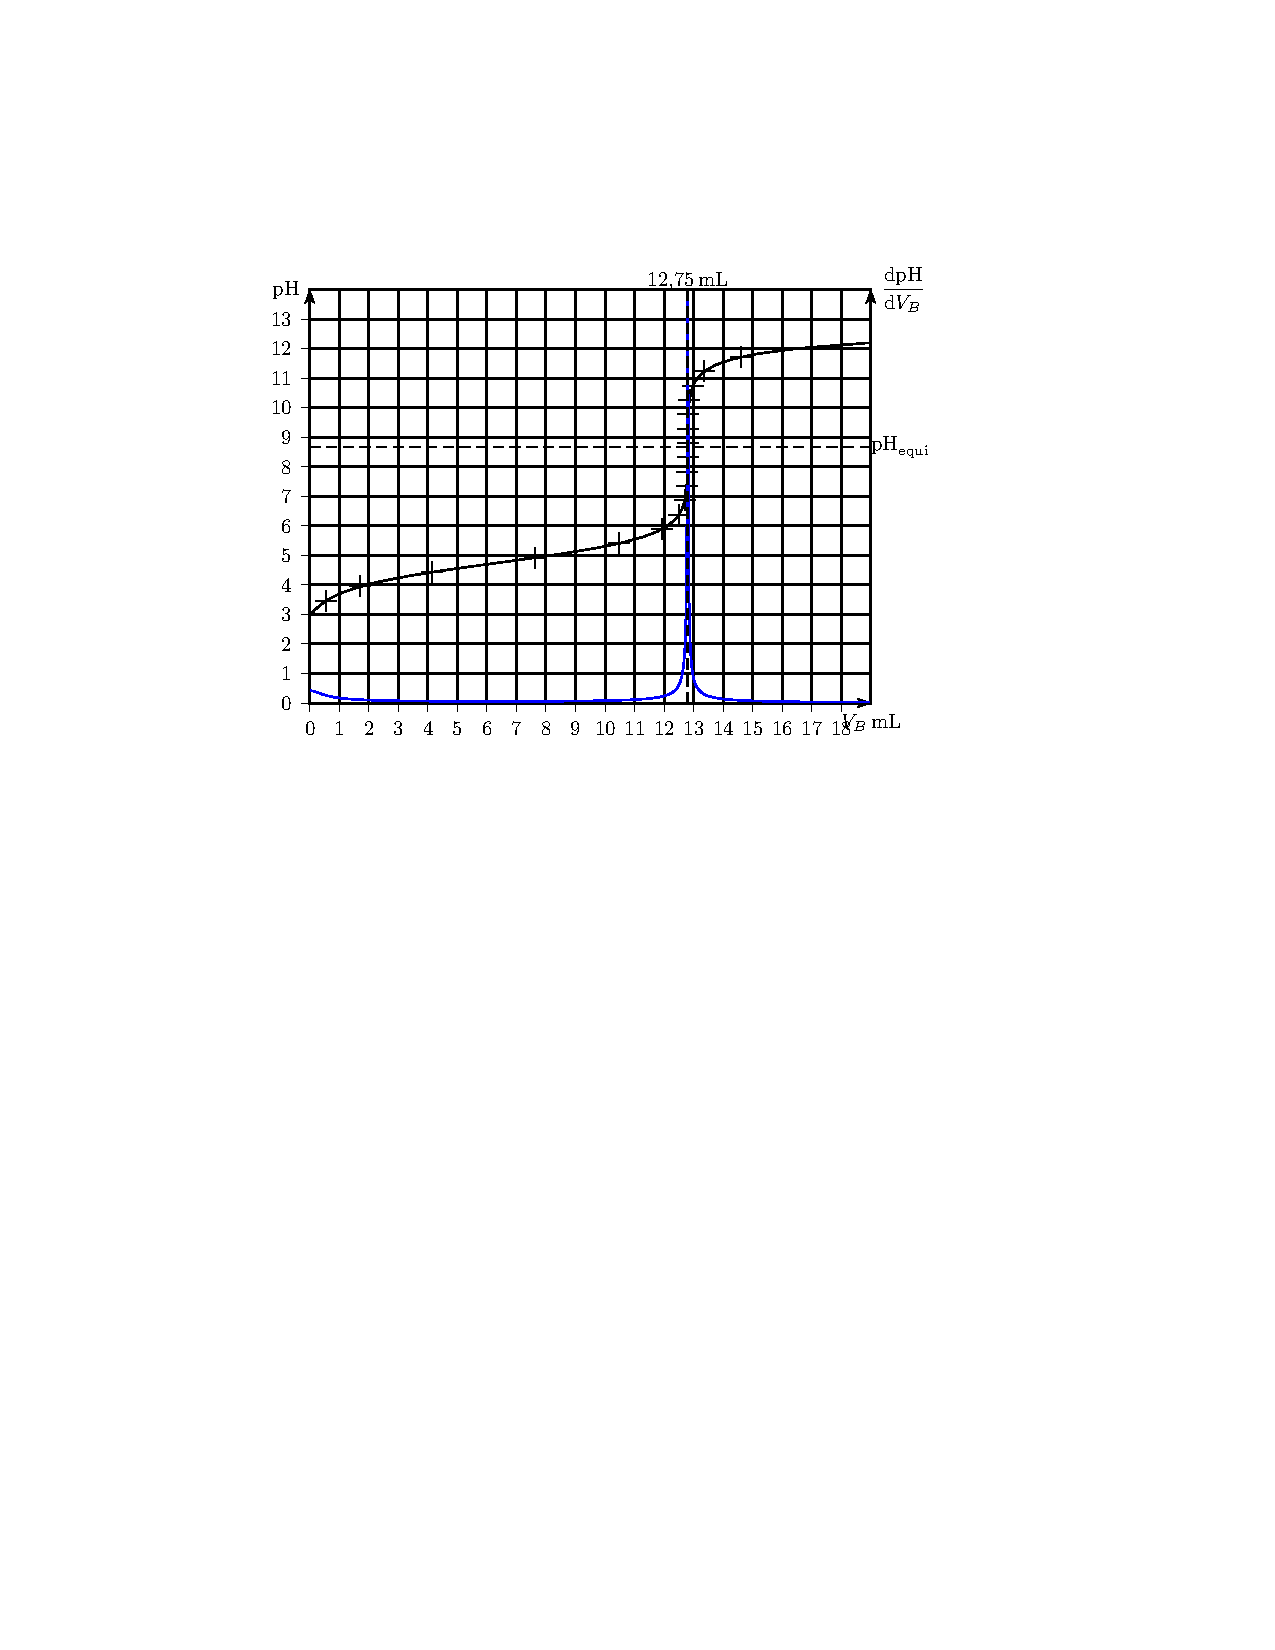
\includegraphics[width=.8\linewidth, valign=t]{vinaigre_titrage-fig1}
	\hspace*{\fill}
}

\QR{%
	Donner la relation à l'équivalence. On notera $c_1$ la concentration
	en acide acétique du vinaigre dilué de la solution $S_1$. En déduire la
	concentration $c_0$ de la solution commerciale.
}{%
	Avec un tableau d'avancement, on obtient~:
	\[
		c_1V_A = c_B V\ind{equi}
		\Lra
		\boxed{c_0 = 10 \frac{c_B V\ind{equi}}{V_A}}
		\Ra
		\xul{c_0 = \SI{1.30}{mol.L^{-1}}}
	\]
}

\QR{%
	Calculer l'écart \textbf{relatif} sur la concentration commerciale.
}{%
	\ifstudent{
		\leavevmode\vspace*{-20pt}\relax
	}
	% Avec $u(V\ind{equi}) = \SI{0.1}{mL}$, on a $u(c_{0, \exp}) =
	% \SI{123}{mol.L^{-1}}$~:
	% \[
	% \boxed{E_N = \frac{\abs{c_{0, \exp} - c_{0, \rm theo}}}{u(c_{0, \exp})}}
	% \Lra
	% \xul{E_N = \num{0.5}}
	% \]
	\[
		\boxed{\ep_r = \frac{\abs{c_{0, \exp} - c_{0, \rm theo}}}{c\ind{theo}}}
		\Lra
		\xul{\ep_r = \num{0.05}}
	\]
}

\subsection{Dosage pH-métrique par suivi colorimétrique~: choix de l'indicateur}

\enonce{%
	Les indicateurs colorés de pH (ou indicateurs acide-base) sont des molécules qui
	ont la capacité de changer de couleur en fonction de l'acidité de leur milieu
	environnant.

	\begin{tcb}(rapp)<lftt>{Rappel}
		La zone de virage de l'indicateur coloré doit contenir le pH à l'équivalence
		$\pH\ind{eq}$. Ainsi, lors du saut de $\pH$ consécutif au changement de
		réactif limitant, il y a changement franc de la couleur de l'indicateur.
	\end{tcb}

	\begin{table}[h!]
		\centering
		\caption{Indicateurs proposés.}
		\label{tab:ind}
		\begin{tabular}{lccc}
			\toprule
			Indicateur          & Couleur acide & Zone de virage       & Couleur basique
			\\\midrule
			Bleu de bromothymol & jaune         & \SIrange{6.0}{7.6}{} & bleu
			\\
			Rouge de crésol     & jaune         & \SIrange{7.2}{8.1}{} & rouge
			\\
			Hélianthine         & rouge         & \SIrange{3.2}{4.4}{} & jaune
			\\\bottomrule
		\end{tabular}
	\end{table}
}

\QR{%
	Parmi les indicateurs de la table~\ref{tab:ind}, quel indicateur
	coloré faudrait-il choisir pour réaliser un dosage colorimétrique du
	vinaigre~?
}{%
	Il faut que le saut de pH soit le plus proche du pH à l'équivalence, ici
	$\pH\ind{equi} \approx \num{8.75}$. C'est donc le \textbf{rouge de crésol} le
	plus adapté.
}

\enonce{%
	\begin{tcb}[cnt, bld](impo){Important}
		Nous ne réaliserons pas ce dosage.
	\end{tcb}
}

\subsection{Réalisation du dosage par conductimétrie}
\enonce{%
	\subsubsection{Préparation du conductimètre}

	La cellule conductimétrique est constituée de deux lames planes, parallèles, en
	platine platiné (platine recouvert de platine par hydrolyse). Le conductimètre
	mesure la résistance $R$ ou la conductance $G$ de la colonne de solution qui est
	directement proportionnelle à la conductance $\sigma$. La cellule du
	conductimètre est conservée dans un grand bécher contenant de l'eau distillée,
	il ne reste plus qu'à la plonger dans la solution à étudier.
}
\setcounter{subsubsection}{1}

\subsubsection{Dosage}

\enonce{%
	\begin{tcb}*(expe)<itc>"chem"{Dosage}
		\begin{enumerate}
			\item Suivre le même protocole que pour le dosage pH métrique.
			\item Mettre les $\SI{10}{mL}$ de la solution $S_1$ préalablement préparée
			      dans un grand bécher et ajouter de $200$ à $\SI{250}{mL}$ d'eau
			      distillée (la précision du volume n'a aucune importance tant qu'il est
			      suffisant pour pouvoir négliger le volume de solution titrante versé).
		\end{enumerate}
	\end{tcb}
}

\QR{%
	Réaliser les mesures en remplissant un tableau de valeurs permettant
	de tracer $G = f (V_B)$, pour des additions de soude de $0,1,2… \si{mL}$
	jusqu'à ce que $V_B \approx 2 V_{B, \eqi}$.
}{%
	Non corrigé.
}

\subsubsection{Exploitation des mesures}

\enonce{%
	Connectez-vous sur \texttt{Capytale} à l'adresse
	\url{https://capytale2.ac-paris.fr/web/c/cf5a-1487558}, puis~:

	\begin{tcb}*(expe)<lfnt>"code"{Code}
		\begin{enumerate}
			\item Compléter les listes $V$, $G$ de vos valeurs relevées.
			\item Tracer le nuage de points.
			\item Créer les listes de points correspondant aux points avant et après
			      l'équivalence et les tracer sur le graphe correspondant.
			\item Calculez les paramètres des fonctions affines par morceaux ainsi
			      définies, et les tracer.
		\end{enumerate}
	\end{tcb}
}

\QR{%
	Relever à l'aide de la souris le volume de soude
	versé à l'équivalence~: $V_{B, \eqi}$ (comme étant l'intersection des
	modélisations affines), et rentrer sa valeur dans la cellule
	correspondante.
}{%
	Voir~\url{https://capytale2.ac-paris.fr/web/c/87dc-3205315}.
}

\QR{%
	En déduire la concentration $c_1$ en acide acétique de la solution
	$S_1$, puis la concentration $c_0$ de la solution commerciale.
}{%
	Idem.
}

\QR{%
	En déduire le degré alcoolique expérimental du vinaigre.
}{%
	\ifstudent{
		\leavevmode\vspace*{-20pt}\relax
	}
	\[
		d = \frac{m_0}{m_V} = \frac{n_0 M}{m_V} \times \frac{V_V}{V_V}
		\Lra
		\boxed{d = \frac{c_0 M}{\rho_V}}
	\]
}

\QR{%
	Calculer l'écart relatif.
}{%
	\texttt{Capytale}.
}

\section{Valider~: évaluation des incertitudes de mesures}

\enonce{%
	L'objectif est de déterminer l'incertitude-type sur la grandeur $c_1$, que l'on
	notera $u(c_1)$. Cette concentration est obtenue par dosage et s'obtient d'après
	l'expression
	\[
		c_1 = \frac{c_B V_{B,\eqi}}{V_A}
	\]
	L'obtention de $u(c_1)$ va donc être réalisée en deux temps, à effectuer sur
	\texttt{Capytale}~:
	\begin{enumerate}
		\item Détermination de l'incertitude de type B sur les grandeurs $c_B$,
		      $V\ind{Beq}$ et $V_A$. On prendra $u(c_B)/c_B \approx 1 \%$, et vous
		      déterminerez les autres incertitudes, notamment grâce aux indications
		      sur la verrerie.
		\item Détermination de $u(c_1)$ par propagation des incertitudes grâce à la
		      méthode \textsc{Monte-Carlo}.
	\end{enumerate}
}

\QR{%
	En tenant compte des indications précédentes, calculer $u(c_1)$ et
	écrire le résultat du mesurage de $c_1$ sous la forme $M(c_1) = m(c_1)
		\pm u(c_1)$. Vous justifierez les incertitudes de type B que vous avez
	choisi pour $V_{B, \eqi}$ et $V_A$.
}{%
	% TODO: 
}

\QR{%
	En déduire l'écart \textbf{normalisé} sur le degré du vinaigre.
}{%
	% TODO: 
}

\end{document}
